\section{Segunda iteración}

En esta segunda iteración pretendemos mejorar algunos de los aspectos que nos hemos encontrando en la primera, o aspectos que simplemente hemos dejado para después. Comenzaremos con una alternativa al balanceo de datos, y luego probaremos otros tipos tanto de aprendizaje como de modelos.

\subsection{Balanceo de datos}\ \label{sec:i2-balance}

La toma de nuevos datos es costosa y como tenemos relativamente pocos para la cantidad de columnas (las 168 longitudes de onda), el balanceo de datos es esencial. En la primera iteración, intentamos sortear este problema utilizando métricas que tienen en cuenta el balance de los datos. Sin embargo, podemos balancear los datos en dos pasos: \textit{undersampling} y \textit{oversampling}. 

Como su nombre indica, \textit{undersampling} es una técnica para reducir las muestras de la clase mayoritaria, en nuestro caso los granos sin contaminar. Existen varias técnicas para hacer \textit{undersampling}, las cuales comentaremos en la \textit{sección\ \ref{sec:undersampling}}. Por otro lado, el \textit{oversampling} consiste en la creación de datos sintéticos, similares a los reales, para suplir la diferencia de granos. Al igual que con el \textit{undersampling}, existen diversas técnicas que comentaremos más adelante en la \textit{sección\ \ref{sec:oversampling}}.


\subsubsection{\textit{Undersampling}}\ \label{sec:undersampling}

A la hora de balancear los datos, buscamos, de alguna forma, reducir la diferencia en el número de muestras en las diferentes clases. En el paso de \textit{undersampling}, buscamos reducir la cantidad de muestras de las clases mayoritarias, recordamos que nuestro caso lo podemos ver en la \textit{figura\ \ref{fig:unbalance}}. Para ello, debemos de alguna forma determinar qué muestras de las clases mayoritarias son más redundantes para evitar eliminar muestras `críticas'. Comentaremos a continuación diferentes algoritmos que nos ayudan con este paso.

Los algoritmos que hemos decidido utilizar son los de la librería \href{https://imbalanced-learn.org/stable/}{imblearn} que fue diseñada específicamente para los problemas de clasificación sobre \textit{datasets} desbalanceados.\ \cite{3Undersa98:online}

El primer algoritmo que probaremos será \textit{RandomUnderSampler}, el cual consiste en seleccionar un subconjunto aleatorio de datos. Para intentar no eliminar datos importantes como hemos comentado antes, hay otra versión que aplica una de las tres versiones de la heurística \textit{NearMiss}\ \cite{3Undersa98:online}, la cual se basa en el algoritmo \textit{nearest neighbors}:

\begin{enumerate}
    \item La versión \textbf{1} elimina aquellos datos cuya distancia media a sus \textit{N} vecinos más cercanos de la clase minoritaria sea menor.
    \item La versión \textbf{2} es parecida a la \textbf{1}, pero en esta la distancia media se computa sobre los \textit{N} vecinos más lejanos de la clase minoritaria.
    \item La versión \textbf{3} consta de dos pasos, primero de cada elemento de la clase minoritaria selecciona los \textit{M} vecinos más cercanos de la clase mayoritaria. Luego, por cada muestra seleccionada se calcula la distancia media respecto a los \textit{N} vecinos más cercanos de la clase minoritaria y se eliminan los que, de media, estén más alejados.
\end{enumerate}

El algoritmo \textit{Tomek Links} detecta los llamados \textit{Tomek Links}, estos son enlaces entre dos muestras de diferente clase, pongamos \(x\) e \(y\), definidos tal que para cualquier muestra \(z\): 
\[d(x,y) < d(x,z)\ and\ d(x,y) < d(y,z)\], donde \(d(a, b)\) es la distancia entre la muestra \(a\) y \(b\). En resumen, un \textit{Tomek Link} se da entre las muestras de distintas clases más cercanas entre sí. Este algoritmo suele ser bueno a la hora de eliminar ruido en los datos.

\textit{Edited Nearest Neighbours} en resumen elimina las muestras que no se parezcan demasiado a sus vecinos\ \cite{Wil72}. Para ello, comprueba para cada muestra que sus \textit{N} vecinos más cercanos sean de su misma clase, y si no podemos elegir si nos quedamos con la mayoría o si eliminamos todas las muestras.

Podemos ver los resultados de entrenar los modelos básicos que hemos probado anteriormente sobre los \textit{dataset} reducidos con los métodos comentados en la \textit{tabla\ \ref{tab:undersampling-methods}}. Podemos ver que, generalmente, el algoritmo \textit{Near Miss} es el que mejor funciona, aunque cabe destacar que, como podemos ver en la \textit{figura\ \ref{fig:undersampling-methods-balance}}, el algoritmo \textit{Near Miss} reduce mucho más la cantidad de datos. Por lo tanto, tal vez es el que produzca modelos que peor generalizan, vamos a comprobarlo fijándonos en la `tabla expandida' de resultados \textit{tabla\ \ref{tab:near-miss-v2-results}}, (de la cual hemos extraído los resultados de la \textit{tabla\ \ref{tab:undersampling-methods}}, entre otras), podemos ver que los modelos obtienen bastante mejores resultados sobre el dataset de entreno (\textit{Train score}), que sobre el de prueba (\textit{Test score}), por lo tanto sí que hay mucho \textit{overfitting}. Por otro lado, podemos ver que los segundos mejores resultados, los de entrenar utilizando \textit{Edited Nearest Neighbours (ALL)} en la \textit{tabla\ \ref{tab:nearest-neighbors-all-results}}, nos dan modelos que hacen menos \textit{overfitting}. Por lo tanto, nos quedaremos con el para los siguientes pasos. 

\begin{table}[!ht]
    \resizebox{\textwidth}{!}{\begin{tabular}{|c|ccc|} \hline
        & Avg. f0.5 Score & Avg. f2 Score & Avg. Balanced Accuracy \\ \hline
        Random Under Sampler & 61.0523 & 59.2609 & 62.6545 \\
        Near Miss (v1) & 70.2289 & 66.7329 & 69.6297 \\
        \textit{\textbf{Near Miss (v2)}} & 74.6031 & 68.1454 & 73.0865 \\
        Near Miss (v3) & 67.7945 & 71.1278 & 64.9608 \\
        \textit{\textbf{Edited Nearest Neighbors (ALL)}} & 48.8632 & 47.0348 & 67.8832 \\
        Edited Nearest Neighbors (MODE) & 44.4157 & 41.1859 & 64.5333 \\
        Tomek Links & 41.5187 & 41.1415 & 64.6431 \\ \hline
        \end{tabular}}
    \caption{Resultado de entrenar los modelos básicos sobre el \textit{dataset} reducido con los diferentes métodos. Fuente: propia.}\ \label{tab:undersampling-methods}
\end{table}

\begin{table}[!ht]
    \resizebox{\textwidth}{!}{\begin{tabular}{|c|cccc|ccccc|} \hline
        Model Name & Train score & Test score & Recall & Precision & f1score & f0.5score & f2score & ROC/AUC score & Balanced accuracy \\ \hline
        XGBoost & 78.601 & 69.136 & 53.086 & 78.182 & 63.235 & 71.429 & 56.728 & 69.136 & 69.136 \\
        Stochastic Gradient Descent & 66.461 & 53.704 & 44.444 & 54.545 & 48.98 & 52.174 & 46.154 & 53.704 & 53.704 \\
        Random Forest & 100 & 82.099 & 72.84 & 89.394 & 80.272 & 85.507 & 75.641 & 82.099 & 82.099 \\
        Quadratic Discriminant Analysis & 99.794 & 80.247 & 75.309 & 83.562 & 79.221 & 81.769 & 76.826 & 80.247 & 80.247 \\
        Multi-Layer Perceptron & 98.148 & 79.63 & 76.543 & 81.579 & 78.981 & 80.519 & 77.5 & 79.63 & 79.63 \\
        Linear Discriminant Analysis & 84.362 & 65.432 & 56.79 & 68.657 & 62.162 & 65.903 & 58.824 & 65.432 & 65.432 \\
        LightGBM & 73.868 & 62.963 & 55.556 & 65.217 & 60 & 63.025 & 57.252 & 62.963 & 62.963 \\
        K-Neighbors & 100 & 85.802 & 77.778 & 92.647 & 84.564 & 89.235 & 80.357 & 85.802 & 85.802 \\
        Extra Trees & 100 & 87.037 & 76.543 & 96.875 & 85.517 & 91.988 & 79.897 & 87.037 & 87.037 \\
        Decision Tree & 73.251 & 64.815 & 75.309 & 62.245 & 68.156 & 64.482 & 72.275 & 64.815 & 64.815 \\ \hline
        \textbf{AVERAGES} & 87.4485 & 73.0865 & & & & 74.6031 & 68.1454 & & 73.0865 \\ \hline
        \end{tabular}}
    \caption{Resultados de entrenar los modelos básicos habiendo reducido los datos con el algoritmo \textit{Near Miss v2}. Fuente propia.}\ \label{tab:near-miss-v2-results}
\end{table}


\begin{table}[!ht]
    \resizebox{\textwidth}{!}{\begin{tabular}{|c|cccc|ccccc|} \hline
        Model Name & Train score & Test score & Recall & Precision & f1score & f0.5score & f2score & ROC/AUC score & Balanced accuracy \\\hline
        XGBoost & 81.633 & 81.674 & 0 & 0 & 0 & 0 & 0 & 50 & 50 \\
        Stochastic Gradient Descent & 60.544 & 56.335 & 53.086 & 21.717 & 30.824 & 24.628 & 41.188 & 55.075 & 55.075 \\
        Random Forest & 100 & 89.14 & 43.21 & 94.595 & 59.322 & 76.419 & 48.476 & 71.328 & 71.328 \\
        Quadratic Discriminant Analysis & 95.843 & 86.878 & 61.728 & 64.935 & 63.291 & 64.267 & 62.344 & 77.125 & 77.125 \\
        Multi-Layer Perceptron & 90.627 & 86.199 & 33.333 & 79.412 & 46.957 & 62.212 & 37.709 & 65.697 & 65.697 \\
        Linear Discriminant Analysis & 84.656 & 79.864 & 20.988 & 40.476 & 27.642 & 34.137 & 23.224 & 57.031 & 57.031 \\
        LightGBM & 78.307 & 72.172 & 65.432 & 35.811 & 46.288 & 39.376 & 56.144 & 69.558 & 69.558 \\
        K-Neighbors & 100 & 92.308 & 70.37 & 85.075 & 77.027 & 81.662 & 72.89 & 83.8 & 83.8 \\
        Extra Trees & 99.32 & 90.045 & 70.37 & 74.026 & 72.152 & 73.265 & 71.072 & 82.415 & 82.415 \\
        Decision Tree & 57.067 & 60.633 & 76.543 & 28.571 & 41.611 & 32.666 & 57.301 & 66.803 & 66.803 \\ \hline
        \textbf{AVERAGES} & 84.7997 & 79.5248 & & & & 48.8632 & 47.0348 & & 67.8832 \\ \hline
        \end{tabular}}
    \caption{Resultados de entrenar los modelos básicos habiendo reducido los datos con el algoritmo \textit{Edited Nearest Neigbhors (ALL)}. Fuente propia.}\ \label{tab:nearest-neighbors-all-results}
\end{table}

\begin{figure}[!ht]
    \centering
    \begin{subfigure}[b]{0.3\textwidth}
        \centering
        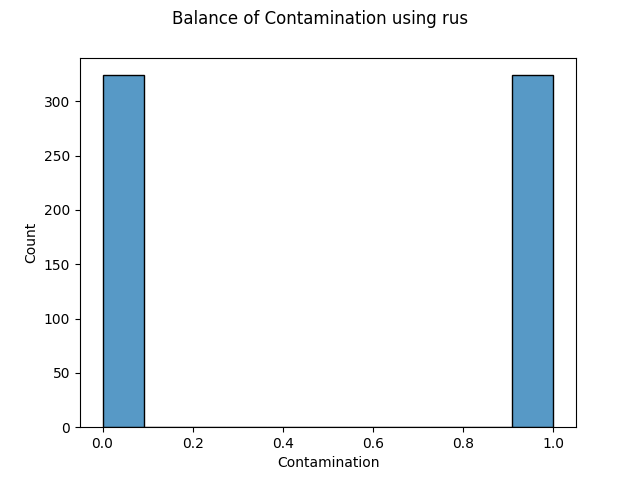
\includegraphics[width=\textwidth]{media/images/under-sampling/rus.png}
        \caption{Balance utilizando \textit{Random Under Sampler}}
    \end{subfigure}
    \begin{subfigure}[b]{0.3\textwidth}
        \centering
        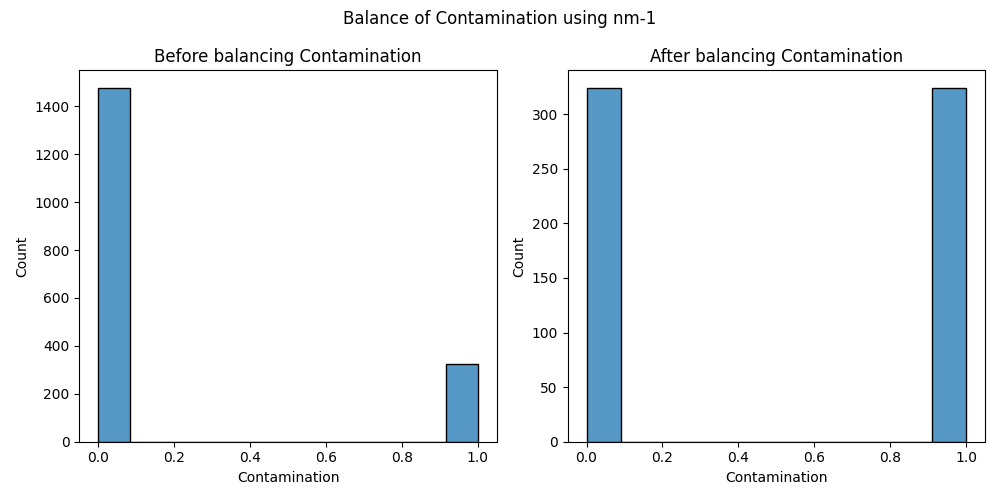
\includegraphics[width=\textwidth]{media/images/under-sampling/nm-1.png}
        \caption{Balance utilizando \textit{Near Miss 1}}
    \end{subfigure}
    \begin{subfigure}[b]{0.3\textwidth}
        \centering
        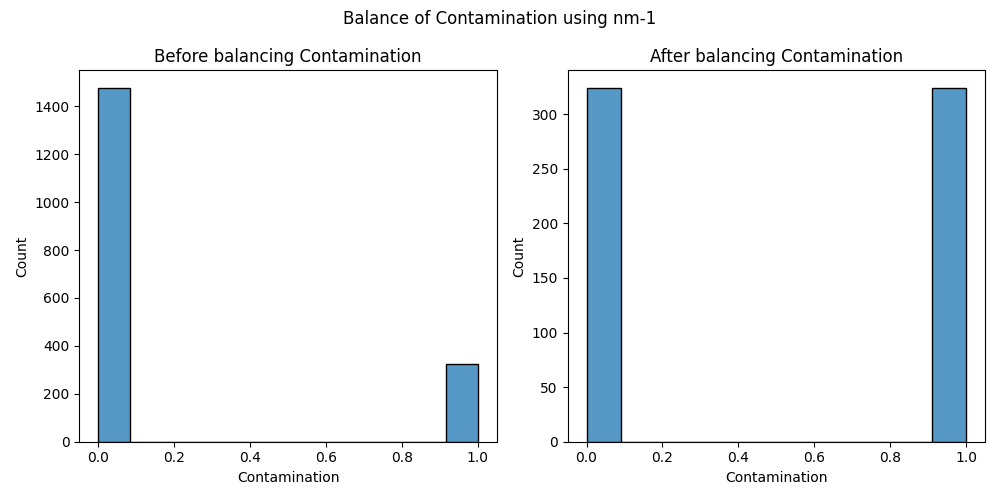
\includegraphics[width=\textwidth]{media/images/under-sampling/nm-1.png}
        \caption{Balance utilizando \textit{Near Miss 2}}
    \end{subfigure}
    \begin{subfigure}[b]{0.3\textwidth}
        \centering
        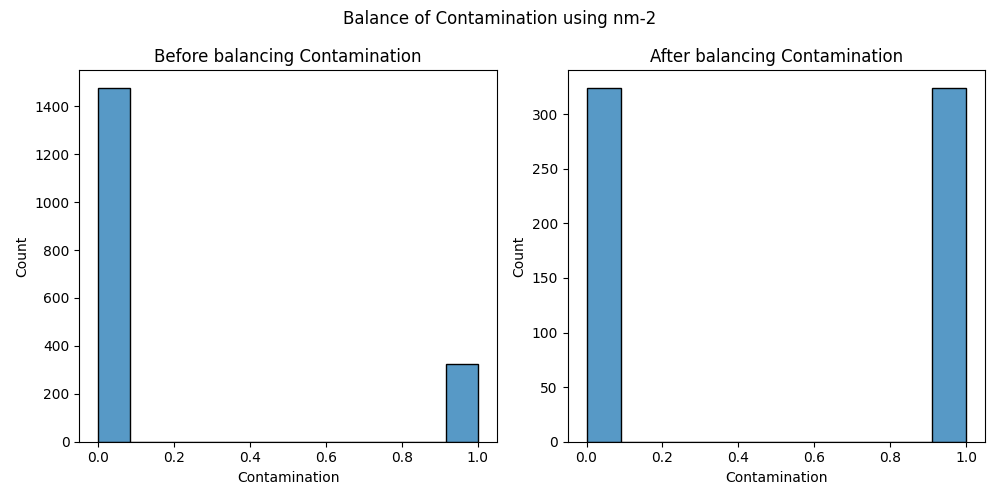
\includegraphics[width=\textwidth]{media/images/under-sampling/nm-2.png}
        \caption{Balance utilizando \textit{Near Miss 3}}
    \end{subfigure}
    \begin{subfigure}[b]{0.3\textwidth}
        \centering
        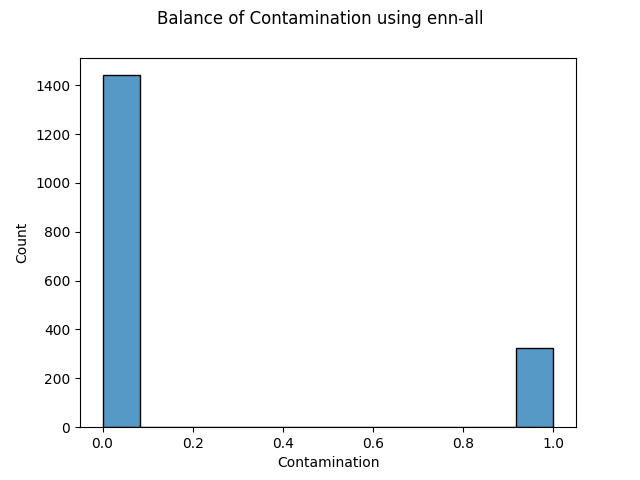
\includegraphics[width=\textwidth]{media/images/under-sampling/enn-all.png}
        \caption{Balance utilizando \textit{Edited Nearest Neighbors (ALL)}}
    \end{subfigure}
    \begin{subfigure}[b]{0.3\textwidth}
        \centering
        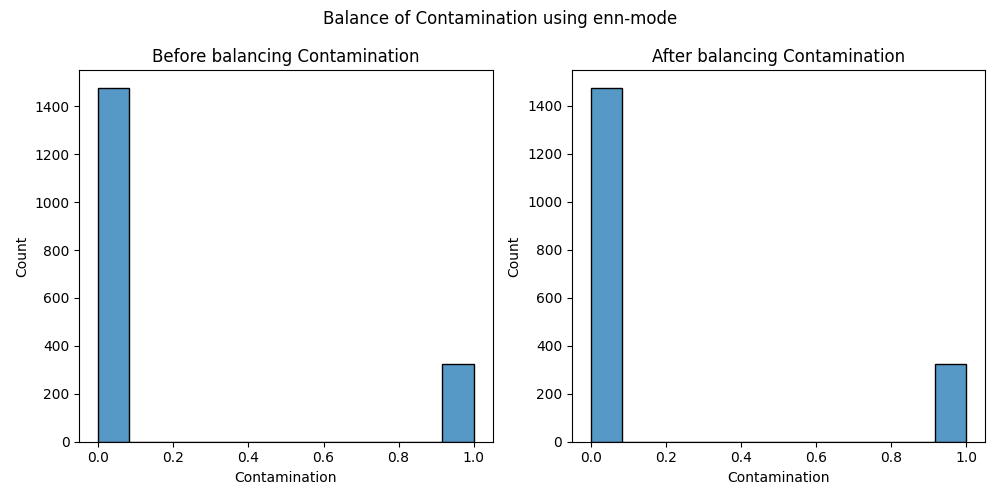
\includegraphics[width=\textwidth]{media/images/under-sampling/enn-mode.png}
        \caption{Balance utilizando \textit{Edited Nearest Neighbors (MODE)}}
    \end{subfigure}
    \begin{subfigure}[b]{0.3\textwidth}
        \centering
        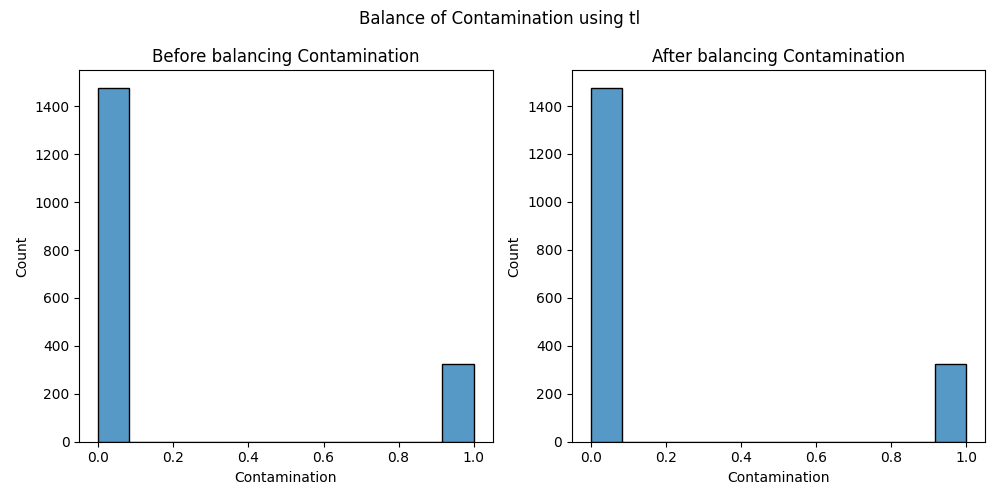
\includegraphics[width=\textwidth]{media/images/under-sampling/tl.png}
        \caption{Balance utilizando \textit{Tomek Links}}
    \end{subfigure}
    \caption{Comparaciones del balance de los \textit{dataset} utilizando los diferentes algoritmos de \textit{undersampling}.}\label{fig:undersampling-methods-balance}
\end{figure}
\clearpage

\subsubsection{\textit{Oversampling}}\ \label{sec:oversampling}

El segundo paso es el \textit{oversampling}, el cual consiste en la creación de los datos sintéticos para suplir la carencia de datos de una clase minoritaria. Hay algoritmos para realizar estas técnicas implementados en \textit{imblearn}, sin embargo preferimos utilizar \href{https://sdv.dev/}{sdv}, pues tiene mejor documentación y tiene un método `fácil' para evaluar los datos generados. \cite{Synthesi69:online} En general, los sintetizadores utilizan algoritmos complejos sobre los cuales podemos leer en \cite{Synthesi69:online}, pero para agilizar el proceso de análisis no entraremos demasiado en detalle.

Antes de comentar los sintetizadores que probaremos, definiremos el método con los que los evaluaremos los datos generados. Utilizaremos una función de la propia librería \textit{sdv} que evalúa la similitud estadística de los datos generados con los datos reales y nos genera un \textit{quality report}.

Los tres sintetizadores que probaremos son:

\begin{enumerate}
    \item \textit{Gaussian Copula Synthesizer} \cite{Gaussian4:online}, el cual utiliza unos métodos clásicos estadísticos.
    \item \textit{CTGANSynthesizer} \cite{CTGANSyn50:online}, utiliza métodos de \textit{deep learning} basados en \textit{GAN} \cite{Generati72:online}.
    \item \textit{TVAESynthesizer} \cite{TVAESynt0:online}, basado en \textit{VAE} \cite{Variatio61:online}, utiliza técnicas de redes neuronales.
\end{enumerate}

Una vez hemos entrenado los sintetizadores, evaluamos su similitud con los datos reales y obtenemos los resultados de la \textit{tabla\ \ref{tab:oversampling-quality-report}}, en los cuales podemos ver un claro `ganador'.

\begin{table}[!ht]
    \centering
    \resizebox{0.8\linewidth}{!}{\begin{tabular}{|c|ccc|} \hline
        Synthesizer & Column Shapes & Column Pair Trends & Overall Quality \\ \hline
        Gaussian Copula Synthesizer & 94.45 & 99.63 & 97.04 \\
        TVAE Synthesizer & 81.59 & 76.19 & 78.89 \\ 
        CTGAN Synthesizer & 73.78 & 54.83 & 64.31 \\ \hline
    \end{tabular}}
    \caption{Resultados del \textit{quality report} de los datos generados con los sintetizadores. Fuente propia}\ \label{tab:oversampling-quality-report}
\end{table}

Ahora que tenemos el mejor \textit{undersampler} y \textit{oversampler} (que hayamos probado para nuestro problema), después de aplicar ambos nos queda el \textit{dataset} con la clase objetivo balanceada como en la \textit{figura\ \ref{fig:balance-second-iteration}}, con el cual podemos entrenar los modelos básicos (aplicando el preprocesado que encontramos en la primera iteración) y obtener los resultados de la \textit{tabla\ \ref{tab:balanced-basic-training}}. 

\begin{figure}[!ht]
    \centering
    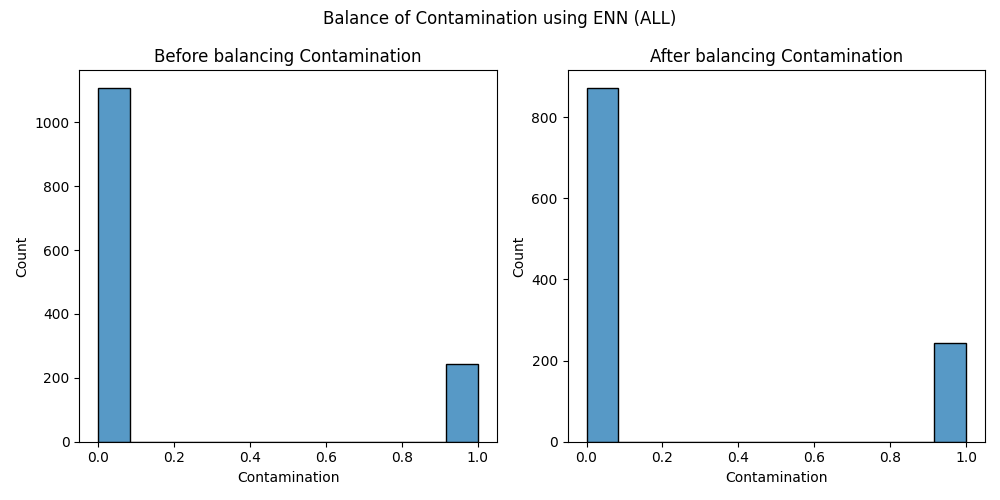
\includegraphics[width=0.7\linewidth]{media/images/balance.png}
    \caption{Comparación del balance de la clase objetivo antes y después de utilizar el método de \textit{undersampling} y \textit{oversampling} comentados. Fuente propia.}\ \label{fig:balance-second-iteration}
\end{figure}

\begin{table}[!ht]
    \centering
    \resizebox{\textwidth}{!}{\begin{tabular}{|c|cccc|ccccc|} \hline
        Model Name & Train score & Test score & Recall & Precision & f1score & f0.5score & f2score & ROC/AUC score & Balanced accuracy \\ \hline
        XGBoost & 90.375 & 89.043 & 80.055 & 97.635 & 87.976 & 93.528 & 83.046 & 89.055 & 89.055 \\
        Stochastic Gradient Descent & 80.009 & 78.641 & 80.609 & 77.6 & 79.076 & 78.184 & 79.989 & 78.638 & 78.638 \\
        Random Forest & 96.391 & 91.956 & 86.704 & 96.904 & 91.52 & 94.676 & 88.568 & 91.963 & 91.963 \\
        Quadratic Discriminant Analysis & 91.624 & 91.401 & 82.825 & 100 & 90.606 & 96.018 & 85.772 & 91.413 & 91.413 \\
        Multi-Layer Perceptron & 94.54 & 92.372 & 86.704 & 97.812 & 91.924 & 95.369 & 88.719 & 92.38 & 92.38 \\
        Linear Discriminant Analysis & 86.025 & 85.576 & 80.332 & 89.783 & 84.795 & 87.719 & 82.06 & 85.583 & 85.583 \\
        LightGBM & 90.375 & 88.904 & 78.947 & 98.616 & 87.692 & 93.935 & 82.227 & 88.918 & 88.918 \\
        K-Neighbors & 100 & 76.56 & 56.51 & 94.444 & 70.711 & 83.265 & 61.446 & 76.588 & 76.588 \\
        Extra Trees & 90.838 & 90.985 & 84.211 & 97.436 & 90.342 & 94.469 & 86.56 & 90.994 & 90.994 \\
        Decision Tree & 83.48 & 84.466 & 70.36 & 98.069 & 81.935 & 90.909 & 74.574 & 84.486 & 84.486 \\ \hline
        \end{tabular}}
    \caption{Resultados de entrenar los modelos básicos habiendo balanceado el \textit{dataset}. Fuente propia.}\ \label{tab:balanced-basic-training}
\end{table}

\clearpage
\subsection{Nuevos modelos}

Hay dos modelos más complejos que no hemos probado que pueden darnos mejores resultados, estos son \textit{Voting Classifier} y \textit{Bagging Classifier}. El primero, \textit{Voting Classifier}, entrena los modelos que lo componen sobre el \textit{dataset} y, a la hora de predecir, se basa en las predicciones de estos modelos. Es decir, realiza una votación y la clase que más se vote es la que sale como predicción como podemos ver en la \textit{figura\ \ref{fig:voting-classifiers}}. Hay dos tipos de votación, \textit{hard} y \textit{soft}, \textit{hard} utiliza la clase predicha de los modelos, mientras que \textit{soft} suma las probabilidades de las clases a predecir y suele ser más preciso \cite{Ensemble96:online}. 

\begin{figure}[!h]
    \centering
    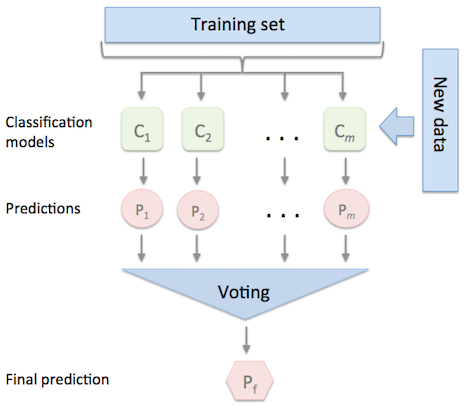
\includegraphics[width=0.7\linewidth]{media/images/majority_voting.png}
    \caption{Explicación gráfica del proceso de entreno y predicción de un \textit{Voting Classifier}. Fuente \cite{Ensemble96:online}.}\ \label{fig:voting-classifiers}
\end{figure}

Por otro lado \textit{Bagging Classifier} entrena el mismo modelo sobre un subconjunto aleatorio del \textit{dataset} y luego agrega los resultados de las predicciones, ya sea haciendo la media o realizando una votación, para obtener una predicción final.\ \cite{sklearne53:online}


Antes de entrenar estos modelos, hemos de decidir qué otros modelos los compondran, por lo tanto, haremos antes un poco de \textit{hyperparameter tuning}, como comentamos en la sección \ref{sec:i1-seleccion}, para tratar de mejorar los modelos base con los que compondremos tanto el \textit{Voting Classifier} como \textit{Bagging Classifier}.

Para hacer \textit{hyperparameter tuning}, seleccionamos primero los modelos que ajustaremos, los cuales son los que mejores resultados han dado del entreno básico, es decir, \textit{Multi-Layer Perceptron, Random Forest, Quadratic Discriminant Analysis y Extra Trees}. De los cuales hemos obtenido los resultados de la \textit{tabla\ \ref{tab:hyperparameter-tuning-results-v2}} donde vemos que tanto \textit{et} como \textit{mlp} han mejorado (aun haciendo \textit{overfitting}), \textit{qda} sigue igual y \textit{rf} ha empeorado. De todas formas, nos sirven los parámetros que hemos encontrado, pues tienen resultados bastante buenos, por lo tanto montaremos tanto el \textit{Voting Classifier} como el \textit{Bagging Classifier} sobre estos.


\begin{table}[!ht]
    \centering
    \resizebox{\textwidth}{!}{\begin{tabular}{|c|ccccccccc|} \hline
        Model name & Train score & Accuracy & Recall & Precision & f1 score & f0.5 score & f2 score & ROC/AUC score & Balanced accuracy \\ \hline
        GS - et & 100 & 95.981 & 93.352 & 98.538 & 95.875 & 97.455 & 94.345 & 95.981 & 95.981 \\
        RS - qda & 91.62 & 91.413 & 82.825 & 100 & 90.606 & 96.018 & 85.772 & 91.413 & 91.413 \\
        GS - qda & 91.62 & 91.413 & 82.825 & 100 & 90.606 & 96.018 & 85.772 & 91.413 & 91.413 \\
        RS - et & 97.778 & 93.487 & 89.474 & 97.289 & 93.218 & 95.619 & 90.935 & 93.487 & 93.487 \\
        RS - mlp & 100 & 94.039 & 91.967 & 95.954 & 93.918 & 95.129 & 92.737 & 94.039 & 94.039 \\
        GS - mlp & 100 & 94.039 & 91.967 & 95.954 & 93.918 & 95.129 & 92.737 & 94.039 & 94.039 \\
        RS - rf & 89.074 & 89.193 & 81.163 & 96.7 & 88.253 & 93.134 & 83.858 & 89.193 & 89.193 \\
        GS - rf & 88.889 & 88.916 & 80.609 & 96.678 & 87.915 & 92.971 & 83.381 & 88.916 & 88.916 \\ \hline
        \end{tabular}}
        \caption{Resultado del \textit{hyperparameter tuning} con el \textit{dataset} balanceado. Fuente propia.}\ \label{tab:hyperparameter-tuning-results-v2}
\end{table}


Al entrenar los \textit{Voting} y \textit{Bagging Classifiers}, obtenemos los resultados de la \textit{tabla\ \ref{tab:voting-bagging-results}}. En general, los \textit{Voting} han obtenido resultados algo mejores que los \textit{Bagging Classifiers}, podría ser por la cantidad de datos sobre los que ha entrenado cada submodelo.

\begin{table}[!ht]
    \centering
    \resizebox{\textwidth}{!}{\begin{tabular}{|c|ccccccccc|} \hline
        Model name & Train score & Accuracy & Recall & Precision & f1 score & f0.5 score & f2 score & ROC/AUC score & Balanced accuracy \\ \hline
        Voting Classifier (All - not tuned) & 100 & 95.839 & 92.244 & 99.403 & 95.69 & 97.884 & 93.592 & 95.844 & 95.844 \\
        Bagging Classifier (QDA) & 96.9 & 95.284 & 90.859 & 99.696 & 95.072 & 97.794 & 92.499 & 95.29 & 95.29 \\
        Voting Classifier (QDA and ET) & 97.501 & 95.007 & 90.028 & 100 & 94.752 & 97.833 & 91.86 & 95.014 & 95.014 \\
        Voting Classifier (All) & 98.103 & 94.868 & 90.305 & 99.39 & 94.63 & 97.43 & 91.986 & 94.875 & 94.875 \\
        Voting Classifier (RF and ET and QDA) & 97.362 & 94.73 & 89.474 & 100 & 94.444 & 97.701 & 91.398 & 94.737 & 94.737 \\
        Voting Classifier (MLP and ET) & 100 & 93.481 & 91.136 & 95.64 & 93.333 & 94.704 & 92.002 & 93.485 & 93.485 \\
        Bagging Classifier (MLP - not tuned) & 92.92 & 90.846 & 85.873 & 95.385 & 90.379 & 93.317 & 87.62 & 90.853 & 90.853 \\
        Bagging Classifier (RF) & 92.041 & 87.933 & 82.548 & 92.547 & 87.262 & 90.358 & 84.371 & 87.941 & 87.941 \\
        Bagging Classifier (ET) & 89.82 & 87.656 & 82.825 & 91.718 & 87.045 & 89.79 & 84.463 & 87.663 & 87.663 \\ \hline
        \end{tabular}}
        \caption{Resultados de entrenar los diferentes \textit{Voting} y \textit{Bagging Classifiers} que hemos preparado con los resultados del \textit{hyperparameter tuning}. Fuente propia.}\ \label{tab:voting-bagging-results}
\end{table}